% !TEX root = ../notes_unsupervisedlearning.tex
% Chapter 13: Reinforcement Learning Fundamentals
%%%%%%%%%%%%%%%%%%%%%%%%%%%%%%%%%%%%%%%%%%%%%%%%%%%%%%%%%%%%%%%%%%%%%%

\chapter{Reinforcement Learning Fundamentals}\index{Reinforcement Learning}\index{DQN}\index{PPO}
\newthought{Learning from rewards, not labels.}

%═══════════════════════════════════════════════════════════════════════
% BLOCK 1: INTRODUCTION
%═══════════════════════════════════════════════════════════════════════

\section{The Why}

\marginnote{Many tasks provide rewards, not labels: games, robotics, trading.}

Supervised learning needs labeled data. But many important tasks only provide sparse feedback:
\begin{itemize}
    \item \textbf{Games}: Win or lose after many moves
    \item \textbf{Robotics}: Task success after many actions
    \item \textbf{Dialogue}: User satisfaction at conversation end
    \item \textbf{Trading}: Profit after many trades
\end{itemize}

\textbf{Reinforcement learning} learns from \textbf{rewards}: scalar feedback indicating how good an action was. The agent must:
\begin{itemize}
    \item Explore to discover good actions
    \item Exploit known good actions for reward
    \item Handle delayed rewards (credit assignment)
\end{itemize}

\subsection{Hands-On Experience}

\begin{marginfigure}
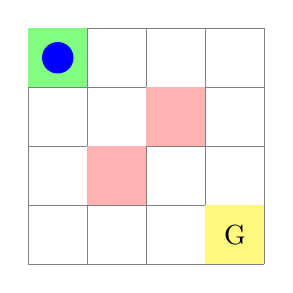
\begin{tikzpicture}[scale=0.5]
    % Grid
    \draw[step=1.5cm, gray, thin] (0,0) grid (6,6);
    % Start
    \fill[green!50] (0,4.5) rectangle (1.5,6);
    \node at (0.75,5.25) {S};
    % Goal
    \fill[yellow!50] (4.5,0) rectangle (6,1.5);
    \node at (5.25,0.75) {G};
    % Obstacle
    \fill[red!30] (1.5,1.5) rectangle (3,3);
    \fill[red!30] (3,3) rectangle (4.5,4.5);
    % Agent
    \fill[blue] (0.75,5.25) circle (0.4);
\end{tikzpicture}
\caption{Gridworld: navigate from S to G, avoiding obstacles.}
\end{marginfigure}

Consider a 4×4 gridworld:
\begin{itemize}
    \item Start at top-left, goal at bottom-right
    \item Actions: up, down, left, right
    \item Reward: $+1$ at goal, $-1$ for hitting obstacle, $0$ otherwise
\end{itemize}

\textbf{Questions}:
\begin{enumerate}
    \item What's the optimal policy?
    \item How would you estimate the value of each state?
    \item What if you didn't know the transition probabilities?
\end{enumerate}

\subsection{Learning Objectives}

After this lecture, you will be able to:
\begin{enumerate}
    \item Formalize problems as Markov Decision Processes (MDPs)
    \item Derive and implement Q-learning and DQN
    \item Explain policy gradient methods and their variance reduction
    \item Apply PPO for stable policy optimization
    \item Choose between value-based and policy-based methods
\end{enumerate}

%═══════════════════════════════════════════════════════════════════════
% BLOCK 2: MAIN THEORY
%═══════════════════════════════════════════════════════════════════════

\section{Markov Decision Processes}

\marginnote{MDPs formalize sequential decision making under uncertainty.}

\begin{definition}[MDP]
A Markov Decision Process is a tuple $(S, A, P, R, \gamma)$:
\begin{itemize}
    \item $S$: State space
    \item $A$: Action space
    \item $P(s'|s,a)$: Transition probability
    \item $R(s,a,s')$: Reward function
    \item $\gamma \in [0,1]$: Discount factor
\end{itemize}
\end{definition}

\textbf{Markov property}: Future depends only on current state, not history:
\begin{equation}
    P(s_{t+1} | s_t, a_t, s_{t-1}, a_{t-1}, \ldots) = P(s_{t+1} | s_t, a_t)
\end{equation}

\subsection{Policies and Value Functions}

\begin{definition}[Policy]
A policy $\pi: S \to \Delta(A)$ maps states to action distributions.
\end{definition}

\begin{definition}[State Value]
\begin{equation}
    V^\pi(s) = \mathbb{E}_\pi \left[ \sum_{t=0}^\infty \gamma^t R_t \mid s_0 = s \right]
\end{equation}
\end{definition}

\begin{definition}[Action Value (Q-function)]
\begin{equation}
    Q^\pi(s,a) = \mathbb{E}_\pi \left[ \sum_{t=0}^\infty \gamma^t R_t \mid s_0 = s, a_0 = a \right]
\end{equation}
\end{definition}

\subsection{Bellman Equations}

\marginnote{Bellman equations: the foundation of RL algorithms.}

\begin{equation}
    V^\pi(s) = \sum_a \pi(a|s) \sum_{s'} P(s'|s,a) [R(s,a,s') + \gamma V^\pi(s')]
\end{equation}

\begin{equation}
    Q^\pi(s,a) = \sum_{s'} P(s'|s,a) [R(s,a,s') + \gamma \sum_{a'} \pi(a'|s') Q^\pi(s',a')]
\end{equation}

\textbf{Optimal} value functions satisfy:
\begin{equation}
    Q^*(s,a) = \sum_{s'} P(s'|s,a) [R(s,a,s') + \gamma \max_{a'} Q^*(s',a')]
\end{equation}


\section{Value-Based Methods}

\marginnote{Learn the Q-function, then act greedily.}

\subsection{Q-Learning}

Update Q-values toward the TD target:
\begin{equation}
    Q(s,a) \gets Q(s,a) + \alpha \left[ r + \gamma \max_{a'} Q(s',a') - Q(s,a) \right]
\end{equation}

\begin{algorithm}[H]
\caption{Q-Learning}
\begin{algorithmic}[1]
\State Initialize $Q(s,a)$ arbitrarily
\For{each episode}
    \State Initialize $s$
    \While{$s$ is not terminal}
        \State Choose $a$ using policy derived from $Q$ (e.g., $\varepsilon$-greedy)
        \State Take action $a$, observe $r$, $s'$
        \State $Q(s,a) \gets Q(s,a) + \alpha [r + \gamma \max_{a'} Q(s',a') - Q(s,a)]$
        \State $s \gets s'$
    \EndWhile
\EndFor
\end{algorithmic}
\end{algorithm}

\textbf{Properties}:
\begin{itemize}
    \item \textbf{Off-policy}: Can learn from any behavior policy
    \item \textbf{Tabular}: Requires enumerable state-action space
    \item \textbf{Convergent}: Under mild conditions, converges to $Q^*$
\end{itemize}


\section{Deep Q-Networks (DQN)}

\marginnote{DQN: Q-learning with neural network function approximation.}

For large/continuous state spaces, use a neural network $Q_\theta(s,a)$:

\begin{equation}
    \mathcal{L}(\theta) = \mathbb{E}_{(s,a,r,s') \sim \mathcal{D}} \left[ (r + \gamma \max_{a'} Q_{\theta^-}(s',a') - Q_\theta(s,a))^2 \right]
\end{equation}

\textbf{Key innovations}:
\begin{enumerate}
    \item \textbf{Experience replay}: Store transitions in buffer $\mathcal{D}$, sample randomly
    \item \textbf{Target network}: Use old parameters $\theta^-$ for target, update periodically
\end{enumerate}

\begin{figure}[h]
\centering
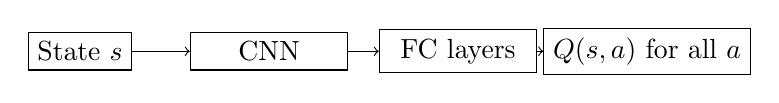
\begin{tikzpicture}[scale=0.8]
    \node[draw, rectangle] (state) at (0,0) {State $s$};
    \node[draw, rectangle, minimum width=2cm] (conv) at (3,0) {CNN};
    \node[draw, rectangle, minimum width=2cm] (fc) at (6,0) {FC layers};
    \node[draw, rectangle] (out) at (9,0) {$Q(s,a)$ for all $a$};

    \draw[->] (state) -- (conv);
    \draw[->] (conv) -- (fc);
    \draw[->] (fc) -- (out);
\end{tikzpicture}
\caption{DQN architecture: CNN processes pixels, outputs Q-value for each action.}
\end{figure}


\section{Policy Gradient Methods}

\marginnote{Directly optimize the policy, not the value function.}

\subsection{Policy Parameterization}

Policy $\pi_\theta(a|s)$ is a neural network outputting action probabilities.

\textbf{Objective}: Maximize expected return:
\begin{equation}
    J(\theta) = \mathbb{E}_{\tau \sim \pi_\theta} \left[ \sum_t \gamma^t r_t \right]
\end{equation}

\subsection{Policy Gradient Theorem}

\begin{equation}
    \nabla_\theta J(\theta) = \mathbb{E}_{\pi_\theta} \left[ \nabla_\theta \log \pi_\theta(a|s) \cdot Q^{\pi_\theta}(s,a) \right]
\end{equation}

\subsection{REINFORCE}

Use Monte Carlo estimate of $Q$:

\begin{algorithm}[H]
\caption{REINFORCE}
\begin{algorithmic}[1]
\For{each episode}
    \State Generate trajectory $\tau = (s_0, a_0, r_0, \ldots)$ using $\pi_\theta$
    \For{each step $t$}
        \State $G_t \gets \sum_{k=t}^\infty \gamma^{k-t} r_k$ \Comment{Return from step $t$}
        \State $\theta \gets \theta + \alpha \gamma^t G_t \nabla_\theta \log \pi_\theta(a_t|s_t)$
    \EndFor
\EndFor
\end{algorithmic}
\end{algorithm}

\textbf{Problem}: High variance due to Monte Carlo estimation.

\subsection{Baseline Subtraction}

Reduce variance by subtracting a baseline $b(s)$:
\begin{equation}
    \nabla_\theta J(\theta) = \mathbb{E} \left[ \nabla_\theta \log \pi_\theta(a|s) \cdot (Q(s,a) - b(s)) \right]
\end{equation}

Using $b(s) = V(s)$ gives the \textbf{advantage}: $A(s,a) = Q(s,a) - V(s)$.


\section{Actor-Critic Methods}

\marginnote{Actor-Critic: combine policy gradient (actor) with value estimation (critic).}

\begin{itemize}
    \item \textbf{Actor}: Policy $\pi_\theta(a|s)$
    \item \textbf{Critic}: Value function $V_\phi(s)$ or $Q_\phi(s,a)$
\end{itemize}

Critic estimates advantage for actor updates:
\begin{equation}
    A(s,a) \approx r + \gamma V_\phi(s') - V_\phi(s)
\end{equation}

\subsection{Generalized Advantage Estimation (GAE)}

\marginnote{GAE balances bias and variance in advantage estimation.}

\begin{equation}
    A_t^{\text{GAE}} = \sum_{l=0}^\infty (\gamma \lambda)^l \delta_{t+l}
\end{equation}

where $\delta_t = r_t + \gamma V(s_{t+1}) - V(s_t)$ is the TD error.


\section{Proximal Policy Optimization (PPO)}

\marginnote{PPO: stable, sample-efficient, widely used.}

\textbf{Problem with vanilla policy gradient}: Large updates can destroy policy.

\textbf{PPO solution}: Clip the objective to limit update size.

\begin{equation}
    \mathcal{L}^{\text{CLIP}}(\theta) = \mathbb{E} \left[ \min\left( r_t(\theta) A_t, \text{clip}(r_t(\theta), 1-\epsilon, 1+\epsilon) A_t \right) \right]
\end{equation}

where $r_t(\theta) = \frac{\pi_\theta(a_t|s_t)}{\pi_{\theta_{\text{old}}}(a_t|s_t)}$ is the probability ratio.

\begin{figure}[h]
\centering
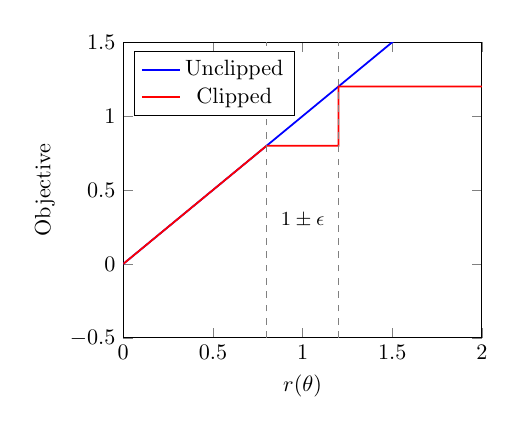
\begin{tikzpicture}[scale=0.8]
    \begin{axis}[
        xlabel={$r(\theta)$},
        ylabel={Objective},
        xmin=0, xmax=2,
        ymin=-0.5, ymax=1.5,
        width=0.6\textwidth,
        legend pos=north west,
    ]
    % Unclipped (A > 0)
    \addplot[blue, thick, domain=0:2] {x};
    % Clipped (A > 0)
    \addplot[red, thick] coordinates {
        (0,0) (0.8,0.8) (0.8,0.8) (1.2,0.8) (1.2,1.2) (2,1.2)
    };
    \draw[dashed, gray] (axis cs:0.8,-0.5) -- (axis cs:0.8,1.5);
    \draw[dashed, gray] (axis cs:1.2,-0.5) -- (axis cs:1.2,1.5);
    \node at (axis cs:1,0.3) {\small $1\pm\epsilon$};
    \legend{Unclipped, Clipped}
    \end{axis}
\end{tikzpicture}
\caption{PPO clipping: prevents too-large policy updates.}
\end{figure}


%═══════════════════════════════════════════════════════════════════════
% BLOCK 3: STUDENT ACTIVATION
%═══════════════════════════════════════════════════════════════════════

\section{Examples \& Exercises}

\subsection{Exercise 1: Q-Learning by Hand}

Gridworld: 3 states (A, B, C). A $\to$ B (r=0), B $\to$ C (r=0), C terminal (r=1). $\gamma = 0.9$, $\alpha = 0.1$.

Initial $Q = 0$ everywhere. Update $Q(B, \text{right})$ after transition $B \to C$.

\textbf{Solution}:
\begin{align*}
    Q(B, \text{right}) &\gets 0 + 0.1 \cdot [0 + 0.9 \cdot \max Q(C, \cdot) - 0] \\
    &= 0.1 \cdot [0 + 0.9 \cdot 0] = 0
\end{align*}

But at terminal $C$, $Q(C, \cdot) = R = 1$! After one more iteration, $Q(B, \text{right}) = 0.09$.

\subsection{Exercise 2: DQN Stability}

Why does DQN need both experience replay and target networks?

\textbf{Solution}:
\begin{itemize}
    \item \textbf{Experience replay}: Breaks correlation between consecutive samples, stabilizes learning
    \item \textbf{Target network}: Prevents moving target problem---without it, both $Q_\theta$ and target change together, causing oscillation
\end{itemize}

\subsection{Exercise 3: Policy Gradient Variance}

REINFORCE has high variance. Why does subtracting a baseline help?

\textbf{Solution}: The gradient $\nabla \log \pi \cdot G$ can be positive or negative depending on $G$. If $G$ is always positive (common in positive-reward environments), all actions get reinforced. Subtracting baseline $V(s)$ centers the signal: good actions (above average) get positive updates, bad actions get negative updates.


\section{Self-Reflection \& Recap}

\subsection{Reflection Questions}
\begin{enumerate}
    \item Why does DQN need experience replay and target networks?
    \begin{quote}
        \textit{Experience replay breaks correlation in training data. Target networks stabilize the bootstrapping target.}
    \end{quote}

    \item When would you prefer policy gradients over Q-learning?
    \begin{quote}
        \textit{Continuous action spaces, stochastic policies, when the optimal policy is simpler than the optimal Q-function.}
    \end{quote}
\end{enumerate}

\subsection{Key Concepts}
\begin{itemize}
    \item \textbf{MDPs} formalize sequential decision problems
    \item \textbf{Q-learning} learns action values via TD updates
    \item \textbf{DQN} scales Q-learning with neural networks
    \item \textbf{Policy gradients} optimize policies directly
    \item \textbf{PPO} provides stable policy optimization via clipping
\end{itemize}

\subsection{Next Chapter Teaser}
\marginnote{Teaser: From trial-and-error to imagination}
\newthought{RL is sample-hungry---learning requires millions of interactions.} What if we could learn a model of the world and plan in imagination? The next chapter explores \textbf{world models} and \textbf{Vision-Language-Action models}---the frontier of embodied AI.
